\clearpage

\section{Práctica 7: Monoestable con LM555}

\subsection{Introducción}

Esta práctica consta de un timer LM555 que es usado como un oscilador monoestable. Este se conecta a un relé, el cuál controla el flujo de corriente hacia un foco de 60W, y un transistor BD135, el cual actúa como un switch para controlar el accionamiento del relé.

El funcionamiento deseado de este circuito es que, después de accionar el botón, pasen 20 segundos, y el relé se accione, permitiendo el paso de corriente hacia el foco y, finalmente, este se encienda. Cabe aclarar que, debido al componente utilizado como timer, este sistema no es reiniciable, es decir, una vez que se presione el botón, no se puede volver a presionar con la intención de que el conteo de los 20 segundos comience de nuevo desde 0. La única de comenzar de nuevo el conteo desde 0 es esperar que pase el primer tiempo, se encieda el foco, y, entonces, se puede presionar el botón para volver a comenzar el ciclo.

\subsection{Objetivos}

Creación de un timer de 20 segundos con un LM555.

\subsection{Marco teórico}

El LM555 es un dispositivo muy estable para generar retardos de tiempo precisos u oscilación. Terminales adicionales son previstas para el disparo o el reajuste si se desea. En el modo de funcionamiento de retardo de tiempo, el tiempo es controlado con precisión por una resistencia externa y capacitor. Para un funcionamiento estable como oscilador, la frecuencia de funcionamiento libre y el ciclo de trabajo se controlan con dos resistencias externas y un condensador. El circuito puede ser disparado y reiniciado en formas de onda descendentes, y el circuito de salida puede o producir hasta 200 mA o manejar circuitos TTL \parencite{texas_instruments_lm555_2015}.

El valor del tiempo que con el que va a trabajar el circuito es definido por medio de una resistencia y un capacitor, siguiendo la siguiente fórmula:
\begin{equation}
    T = 1.1 R_A C_T
    \label{Eq: ecuacion calculo del tiempo}
\end{equation}

El relé SRD-05VDC-Sl-C es  capaz de funcionar hasta con 10 A de corriente circulando a través de él. Está diseñado con un tamaño, principalmente, para su montura en computadoras. El plástico del que está hecho cuenta con una alta resistencia al calor y a sustancias químicas externas. Su funcionamiento se basa en un simple sistema compuesto por una bobina que permite el bajo costo y la producción masiva de este componente. De igual manera, posee dos salidas, para masyor flexibilidad: una normalmente abierta y una normalmente cerrada \parencite{alldatasheet_srd-05vdc-sl-c_nodate}.

El transistor BD135 está montado en el paquete de plástico SOT-32. Está diseñado para amplificadores y controladores de audio que utilizan circuitos complementarios o cuasi-complementarios. Soporta una corriente de base máxima de 500 mA, así como un voltaje emisor-base de 5 V. La ganancia de corriente de este transistor varía dependiendo de la corriente del collector y el voltaje colector-emisor. Posee una ganancia de corriente continua de 250, cuando se utiliza en sus condiciones ideales, es decir, 150 mA de corriente en el colector y 2 V de voltaje colector-emisor \parencite{stmicroelectronics_bd135_nodate}.

\subsection{Circuito}

\begin{figure}[htb]
    \centering
    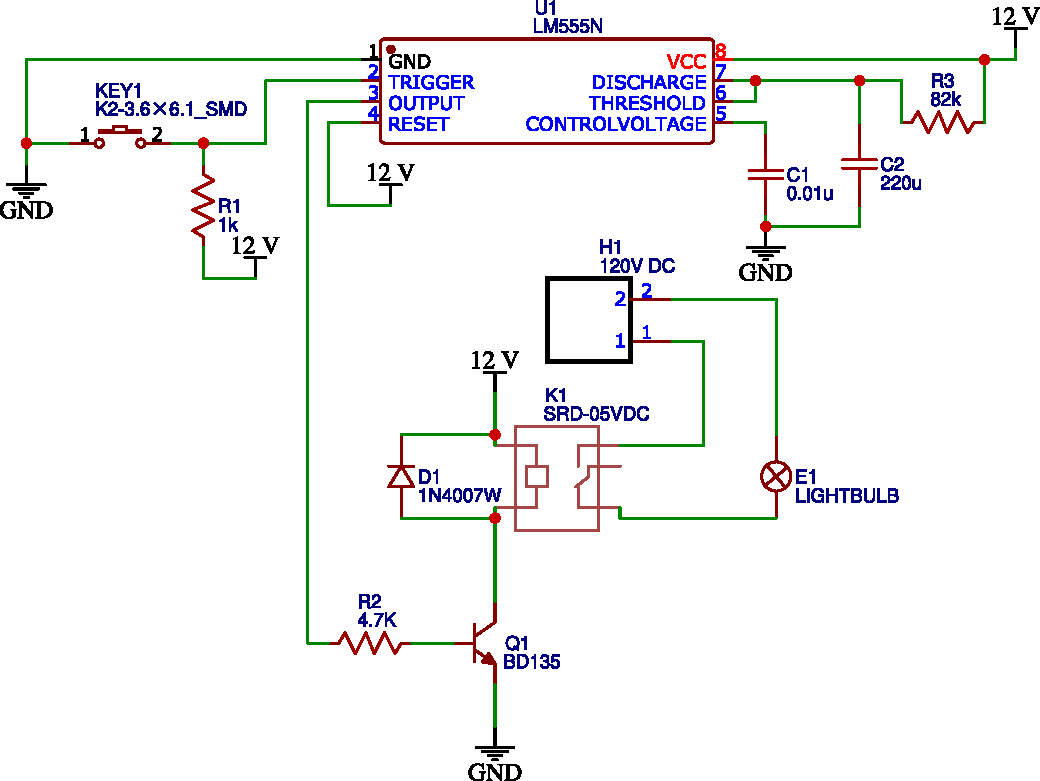
\includegraphics[width=0.8\textwidth]{media/circuito_07}
    \caption{Circuito utilizado en la práctica 7.}
    \label{Fig: Circuito utilizado en la practica 7}
\end{figure}

Tomando en cuenta \eqref{Eq: ecuacion calculo del tiempo} y los valores comerciales de capacitores y resistencias, se obtuvo que el capacitor debe tener un valor de 220 $\mu$F y la resistencia un valor de 82 k$\Omega$ para poder un lograr un tiempo de espera de 19.884 segundos, es decir, praćticamente 20 segundos.

\subsection{Resultados}

\begin{figure}[htb]
    \centering
    \begin{subfigure}[htb]{0.45\textwidth}
        \centering
        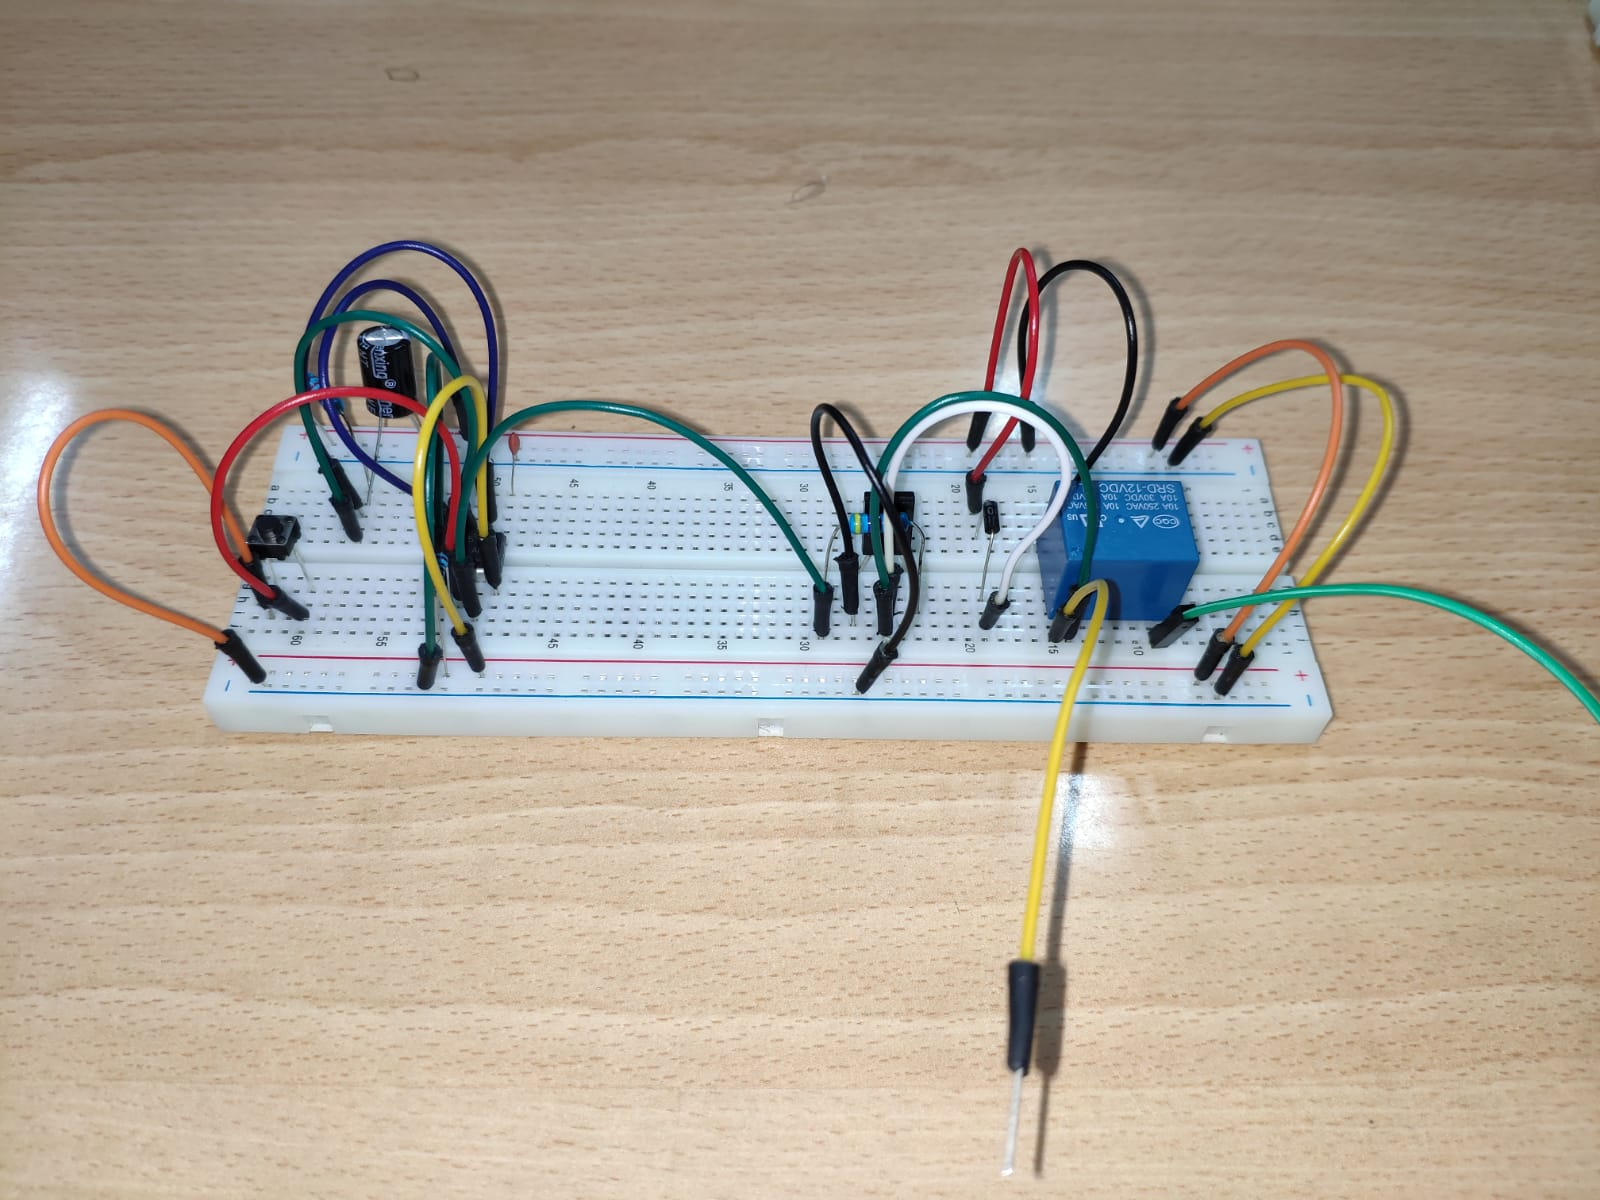
\includegraphics[width=\textwidth]{media/circuito_real_1}
        \caption{}
    \end{subfigure}
    \centering
    \begin{subfigure}[htb]{0.45\textwidth}
        \centering
        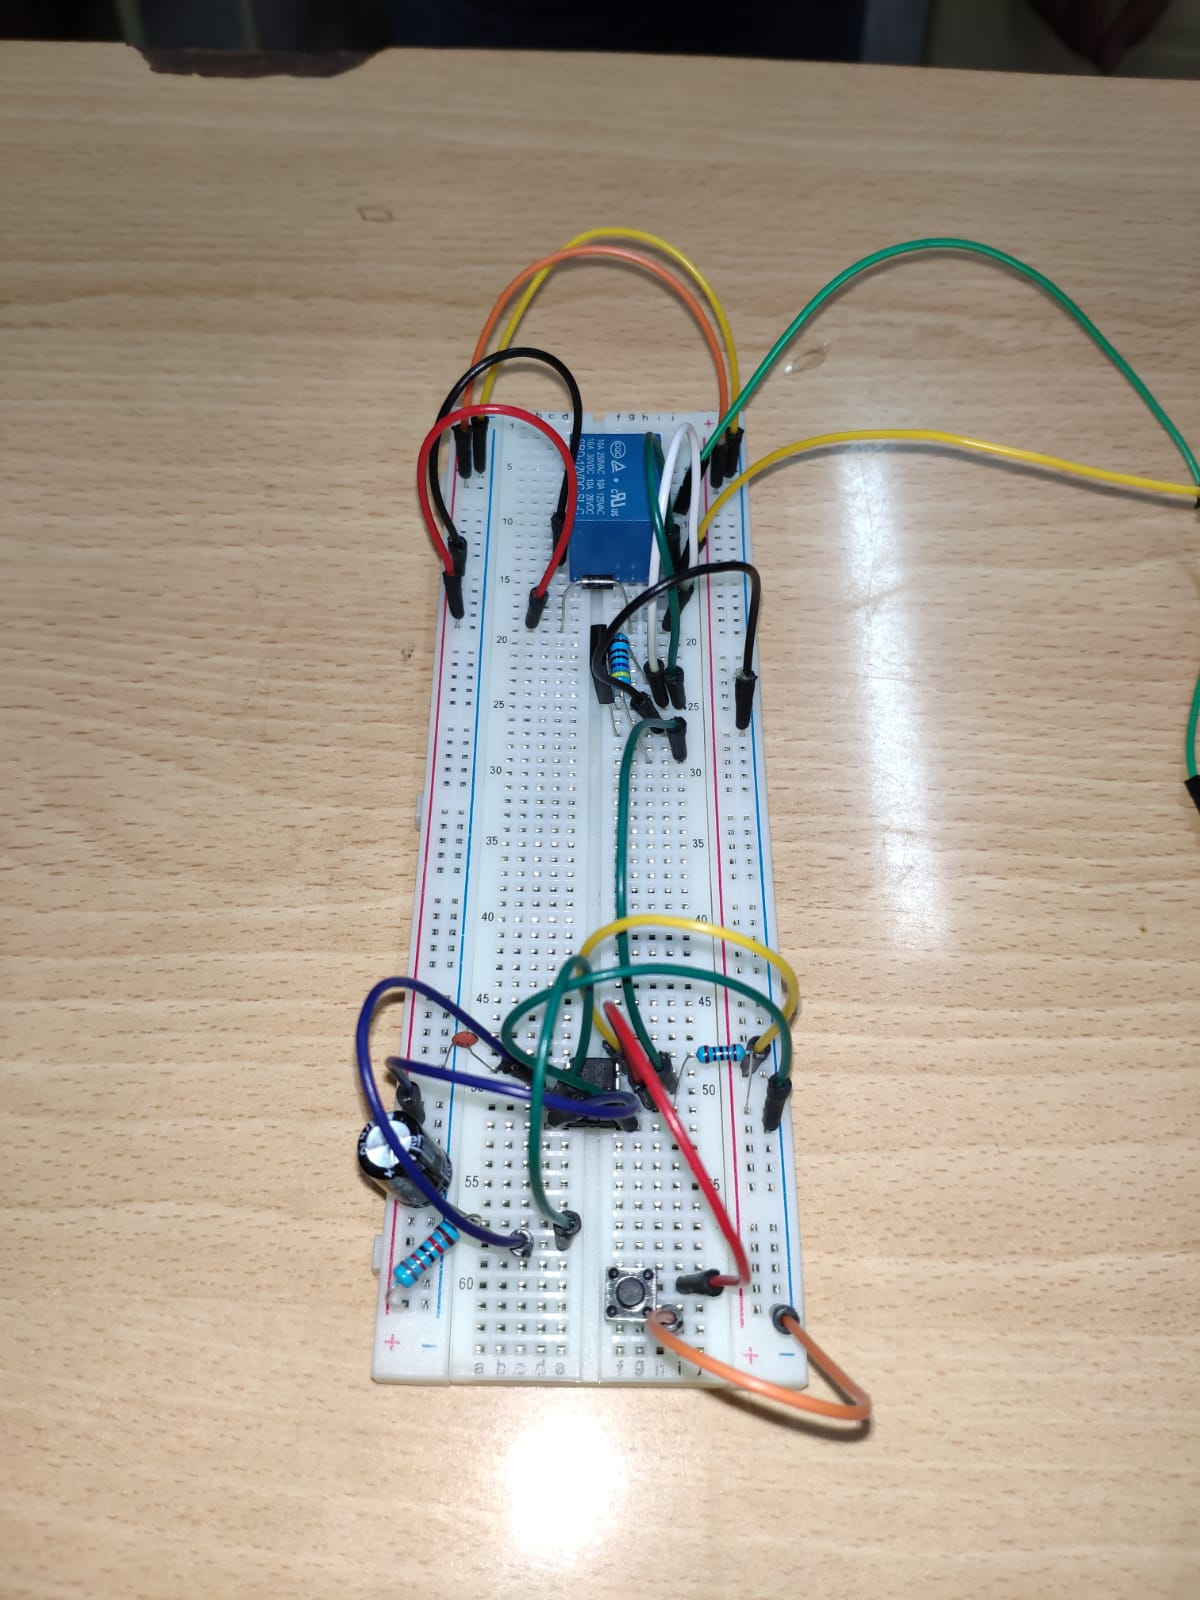
\includegraphics[width=\textwidth]{media/circuito_real_2}
        \caption{}
    \end{subfigure}
    \centering
    \begin{subfigure}[htb]{0.45\textwidth}
        \centering
        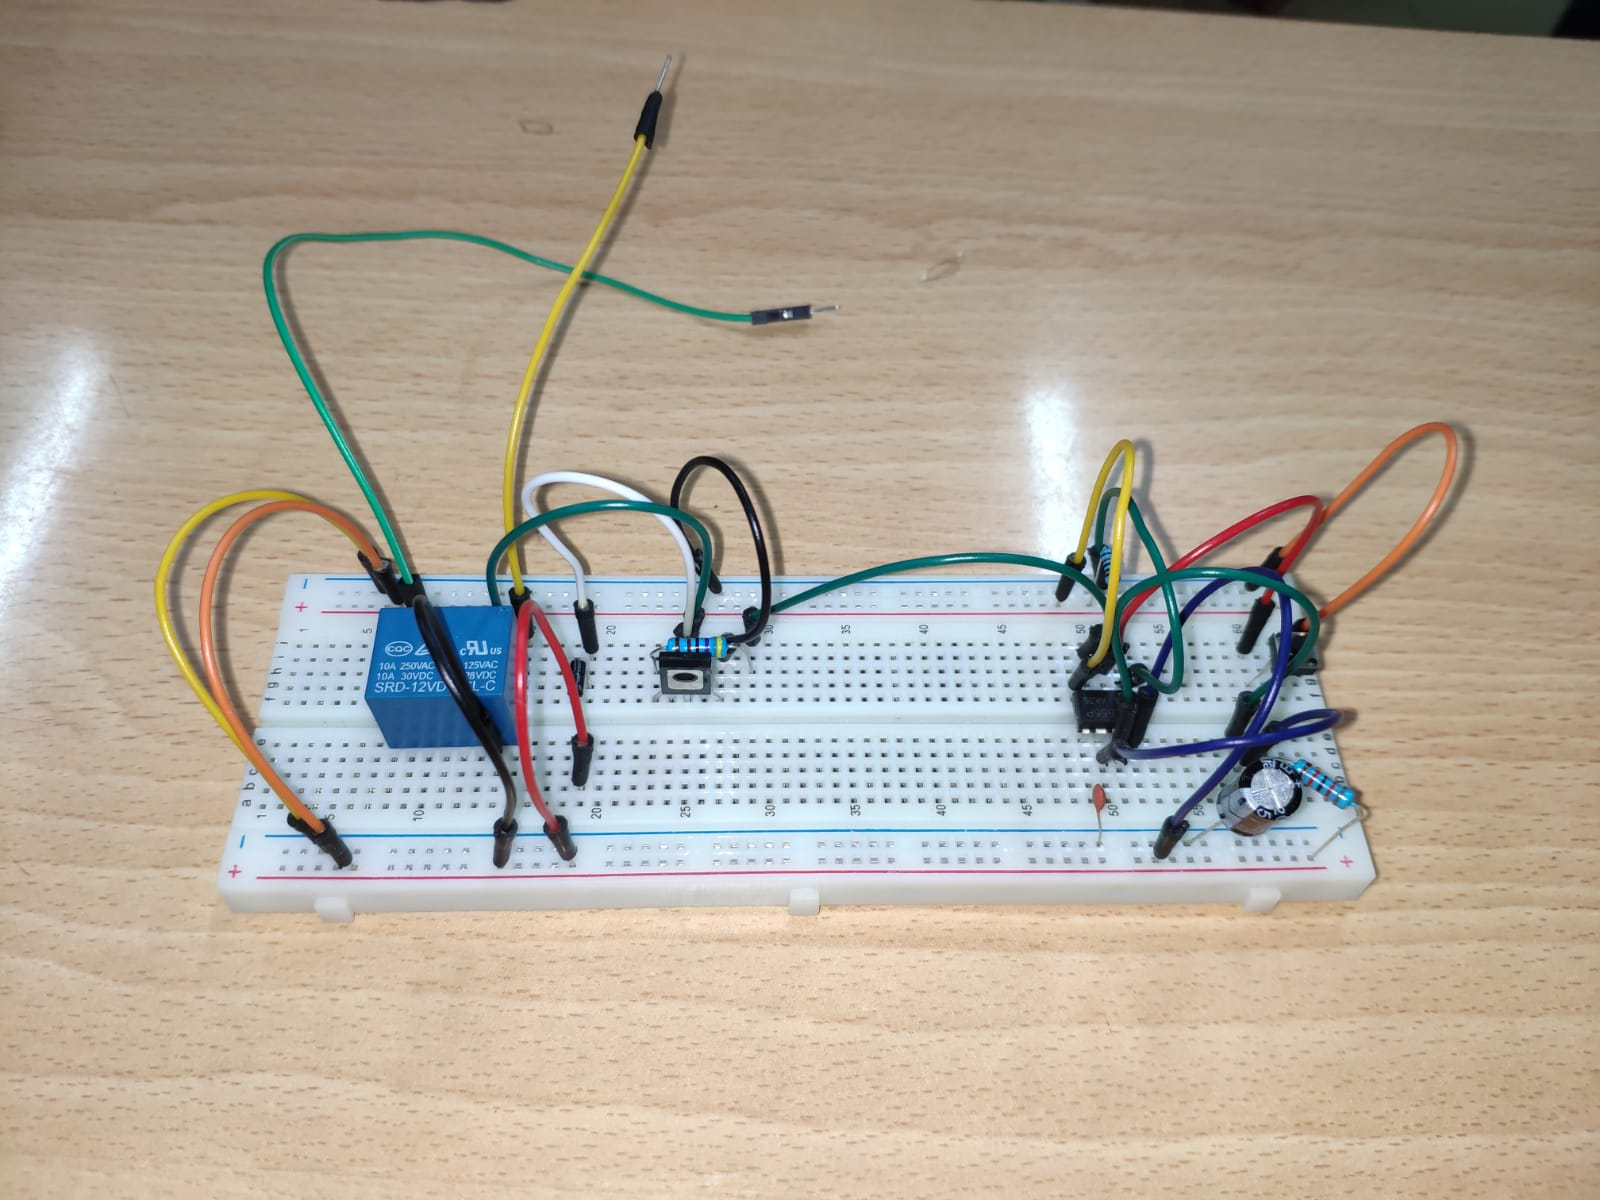
\includegraphics[width=\textwidth]{media/circuito_real_3}
        \caption{}
    \end{subfigure}
    \caption{Fotografías del circuito realizado durante la práctica 7.}
    \label{Fig: Fotografias del circuito realizado durante la practica 7}
\end{figure}

El tiempo del timer que se obtuvo sí fue de 20 segundos, esto debido a que seleccionamos un valor bastante cercano para el cálculo del tiempo de espera por medio de la resistencia y el capacitor, lo que nos permitió tener un valor exacto, aprovechando el LM555. Los valores que tuvimos que cambiar respecto al diagrama mostrado en clase, fueron los voltajes del sistema. En clase el diagrama tenía 5 V de entrada, más, debido al relé que era de 5 V como mínimo, optamos por usar 12 V para la alimenteación, asegurando que el relé siempre recibiera la energía necesaria para activarse cuando recibiera la señal del LM555.

\subsection{Conclusiones}

A pesar de que el LM555 es un timer que tiene dentro de sus características una gran valor de exactitud, el hecho de que no pueda hacerse reseteable lo hace un componente un poco complicado de utilizar en la vida real. Esto debido a que tener un sistema que, una vez accionado, no tenga manera de revertirse, a menos de que se corte la energía, no es realmente una forma de control. Es mejor tener un sistema que sea capaz de controlar este tiempo y poder detenerlo o, como mínimo, poder reiniciarlo, haciéndolo mucho más flexible e, incluso, seguro en sus aplicaciones en sistemas reales.

